% This textfile includes
% 3. Analysis procedures
%    ..
%    ..
%    3.9 Systematic uncertainties

\section{Systematic uncertainties}
The background and signal predictions are affected by systematic uncertainties that have to be estimated and taken into account for limit setting. This section includes a list of the relevant systematic uncertainties for this analysis and how they are estimated.

\begin{itemize}
\item \textbf{Luminosity:} The overall uncertainty of the LHC luminosity delivered to CMS in the 2012 Run-I is measured to be 2.6\%\cite{lumi}
\item \textbf{Jet energy scale:} The systematic on the jet energy scale was studied by scaling up and down the jet mass and $p_{T}$ according to the uncertainty associated to the jet energy corrections used. The Zh mass distributions reconstructed by jet four-momentum is affected and therefore we consider the shape uncertainty as well, shown in Fig.~\ref{fig:SYS_JES}. The overall uncertainty is about 8\%.
\end{itemize}

\begin{figure}[hbtp]
  \centering
  \subfigure[The systematic uncertainty of jet energy scale on background MC $m_{Zh}$ spectrum.]{
    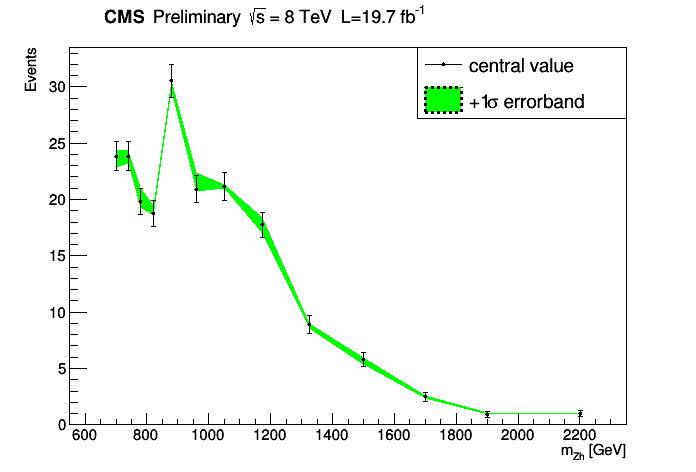
\includegraphics[scale=0.28]{figure/CH3/Systematics/Bkg_jes.png}}
  \hspace{0.5cm}
  \subfigure[The systematic uncertainty of jet energy scale on signal MC $m_{Zh}$ spectrum.]{
    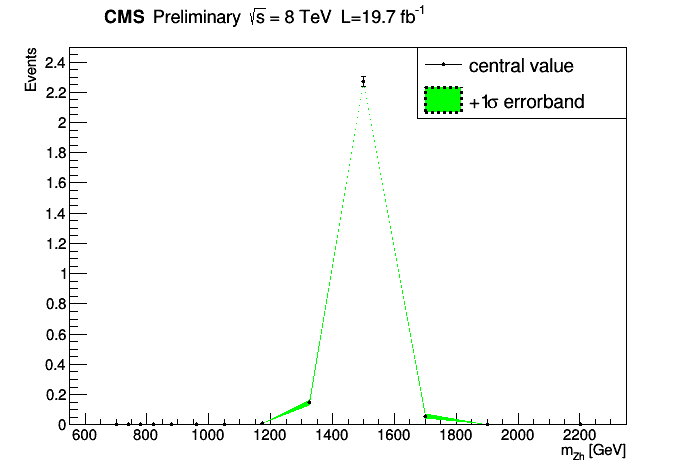
\includegraphics[scale=0.28]{figure/CH3/Systematics/Sig_jes.png}}
  \caption{\label{fig:SYS_JES}SR $m_{Zh}$ distributions for both signal (1500 GeV) and background MC samples. The uncertainty of jet energy scale is shown as the green error band ($\pm1 \sigma$), while the error bar presents the statistic error.}
\end{figure}

\begin{itemize}
\item \textbf{CSV distribution normalization:} The uncertainty comes when normalizing the CSV distributions of MC background prediction in order to match the data distribution, which is estimated about 10\%.
\item \textbf{Pile-up reweighting:} As described previously in section 3.4, we reweight the pile-up interactions in MC predictions for better modeling. To calculate the uncertainties on the pile-up simulation, we produce two pile-up distributions where the minimum bias cross section is shifted by $\pm$5\%\cite{PileupError}. The impact on the event yields is about 2\%. Despite the effects are small, we still consider it as the shape uncertainty. Fig.~\ref{fig:SYS_PU} shows the variation distributions of number of vertices for $\pm1\sigma$.  
\end{itemize}

\begin{figure}[hbtp]
  \centering
  \subfigure[Number of vertices in electron channel.]{
    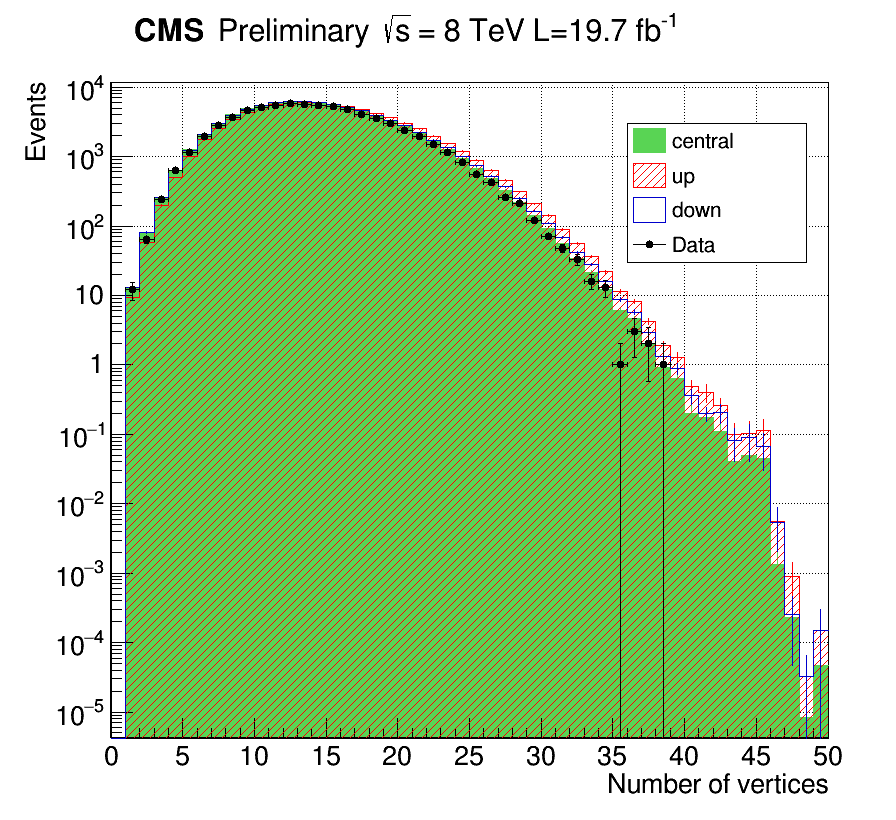
\includegraphics[scale=0.22]{figure/CH3/Systematics/h_nVtx_El_SysLog.png}}
  \hspace{0.5cm}
  \subfigure[Number of vertices in muon channel.]{
    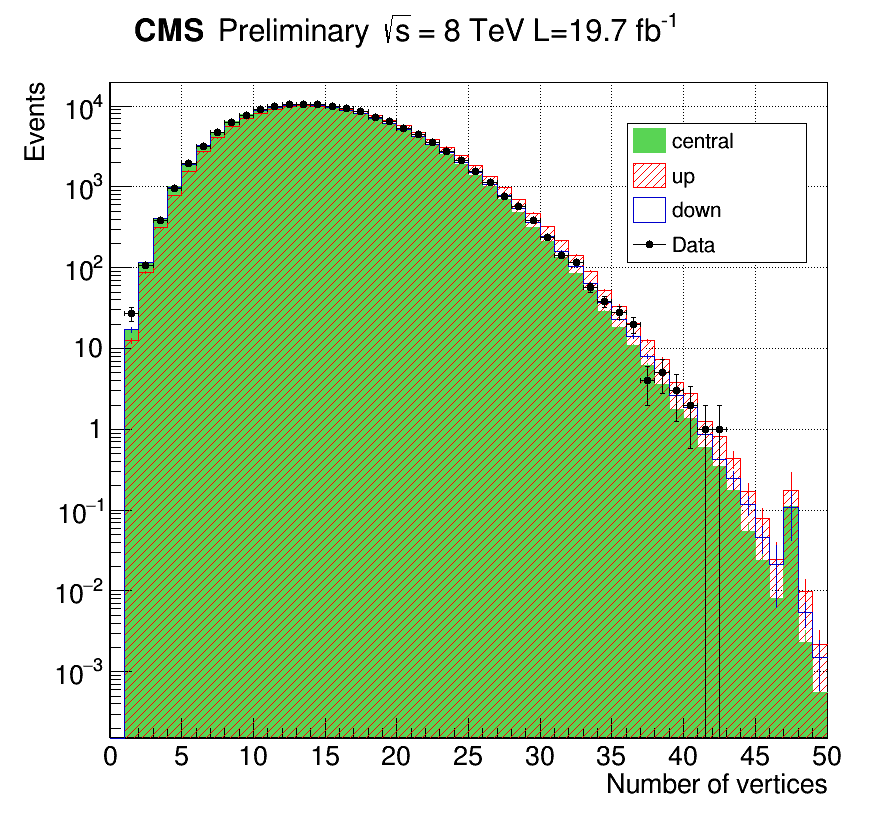
\includegraphics[scale=0.22]{figure/CH3/Systematics/h_nVtx_Mu_SysLog.png}}
  \caption{\label{fig:SYS_PU}(a) shows the distributions of number of vertices in electron channel, comparing central value of the total background prediction and the $\pm1\sigma$ variation, and data as well. (b) shows the result in muon channel.}
\end{figure}

\begin{itemize}
\item \textbf{Lepton ID scale factor:} The muon/electron ID scale factor depends on the kinematics of muon/electron (Table.~\ref{tab:lepIDsf}). This systematic was studied by applying $\pm 1 \sigma$ to the scale factor, the estimated uncertainty is 0.08\% for signal yields, 0.1\% for the Z+jets background, 0.05\% for $t\bar{t}$, and 0.06\% for the SM diboson backgrounds. No shape uncertainties are considered.
\item \textbf{b-jet Ratio:} Since the Drell-Yan process also generates b-jets into our background, the uncertainty of production cross section of Z+b-jets events indeed affects the number of background yield. The cross section ratio defined as $\sigma_{Z+bjet}$ divided by $\sigma_{Z+jet}$ and its uncertainties have been studied in \cite{SMP-13-004}. By scaling $1\sigma$ on the ratio, we etimated there's 0.2\% uncertainty for our Z+jets background yield.
\item \textbf{SHERPA:} The major background sample in this analysis is Z+jets, which is generated by MADGRAPH and showered by PYTHIA. In order to study the dependence on the MC generator, we use the Z+jets sample generated by SHERPA\cite{SHERPA} to estimate the background yield again. The relative uncertainty between SHERPA and MADGRAPH$\times$PYTHIA from the estimated background yield is taken as the systematic by 12\%.
\item \textbf{Diboson cross section:} Uncertainties of the SM WW/WZ/ZZ production cross section affect their estimated background yield about 5.4\%/6.7\%/5.5\%.
\item \textbf{PDF uncertainty:} Systematic uncertainties coming from different choice of PDF sets have been considered for this analysis. This study is performed by varing the PDF set when producing the signal samples. The default PDF set we used is CTEQ6L1, replaced by the following PDF set: MSTW2008lo, MSTW2008nlo, NNPDF21\_lo, NNPDF21\_nlo and CT10. Comparison of distributions from different PDF sets are shown in Fig.~\ref{fig:StackPDF}. The estimated overall uncertainty for signal yields is 12\% (maximum), shape uncertainty is also taken into account.
\end{itemize}

\begin{center}
  \begin{table}[h]
    \begin{center}
      \begin{tabular}{|c|c|c|c|c|}
        \hline
        electron $p_{T}$ [GeV] & $0.0 < |\eta| < 0.8$ & $0.8 < |\eta| < 1.442$ & $1.556 < |\eta| < 2.0$ & $2.0 < |\eta| < 2.5$\\ \hline
        20-30 & 1.005 $\pm$ 0.003 & 0.981 $\pm$ 0.003 & 0.980 $\pm$ 0.005 & 1.017 $\pm$ 0.006\\
        30-40 & 1.004 $\pm$ 0.001 & 0.991 $\pm$ 0.001 & 0.992 $\pm$ 0.002 & 1.019 $\pm$ 0.003\\
        40-50 & 1.008 $\pm$ 0.001 & 0.994 $\pm$ 0.001 & 1.004 $\pm$ 0.002 & 1.005 $\pm$ 0.001\\
        50-200 & 1.008 $\pm$ 0.001 & 0.999 $\pm$ 0.001 & 1.006 $\pm$ 0.003 & 1.009 $\pm$ 0.002\\
        \hline
      \end{tabular}
      \begin{tabular}{|c|c|c|c|}
        \hline
        muon $p_{T}$ [GeV] & $0.0 < |\eta| < 0.8$ & $0.8 < |\eta| < 2.1$ & $2.1 < |\eta| < 2.4$\\ \hline
        20-40 & 1.0043 $\pm$ 0.0004 & 1.0074 $\pm$ 0.0005 & 1.022 $\pm$ 0.001  \\
        40-100 & 1.0012 $\pm$ 0.0004 & 1.0043 $\pm$ 0.0004 & 1.014 $\pm$ 0.001 \\
        \hline
      \end{tabular}
    \end{center}
    \caption{\label{tab:lepIDsf}Data to simulation scale factors for muon and electron identification requirements in various $p_{T}$ and $\eta$ ranges.}
  \end{table}
\end{center}

\begin{figure}[hbtp]
  \centering
  \subfigure[$m_{Zh}$ spectrum of 800 GeV $Z'$ sample]{
    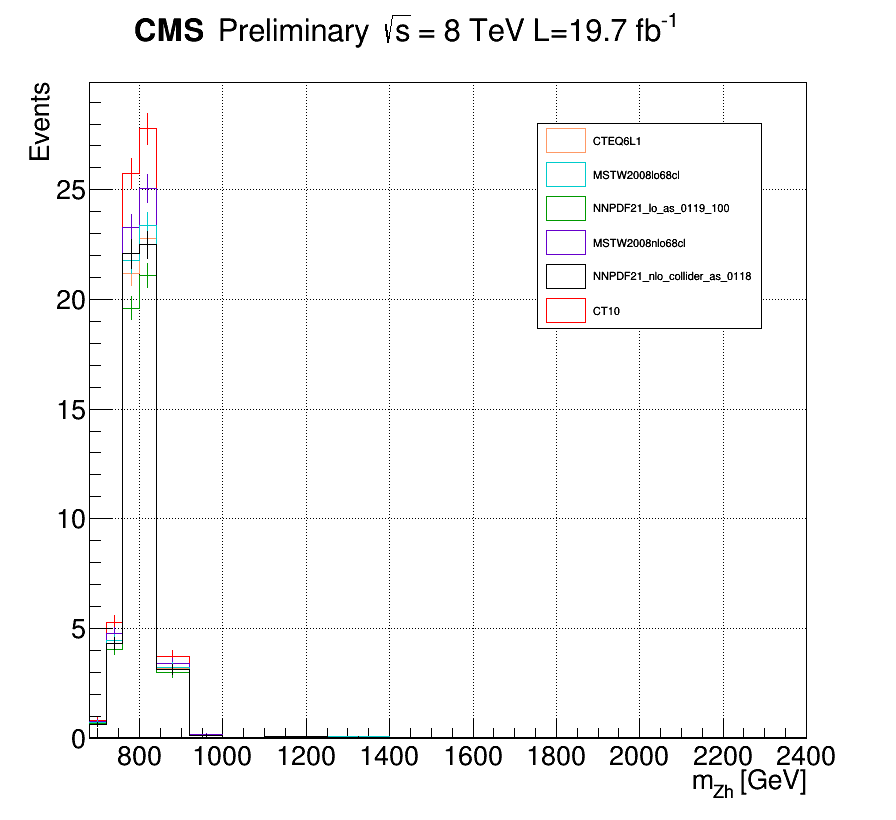
\includegraphics[scale=0.22]{figure/CH3/Systematics/StackPDF_M800.png}}
  \hspace{0.5cm}
  \subfigure[CSV shape of 800 GeV $Z'$ sample]{
    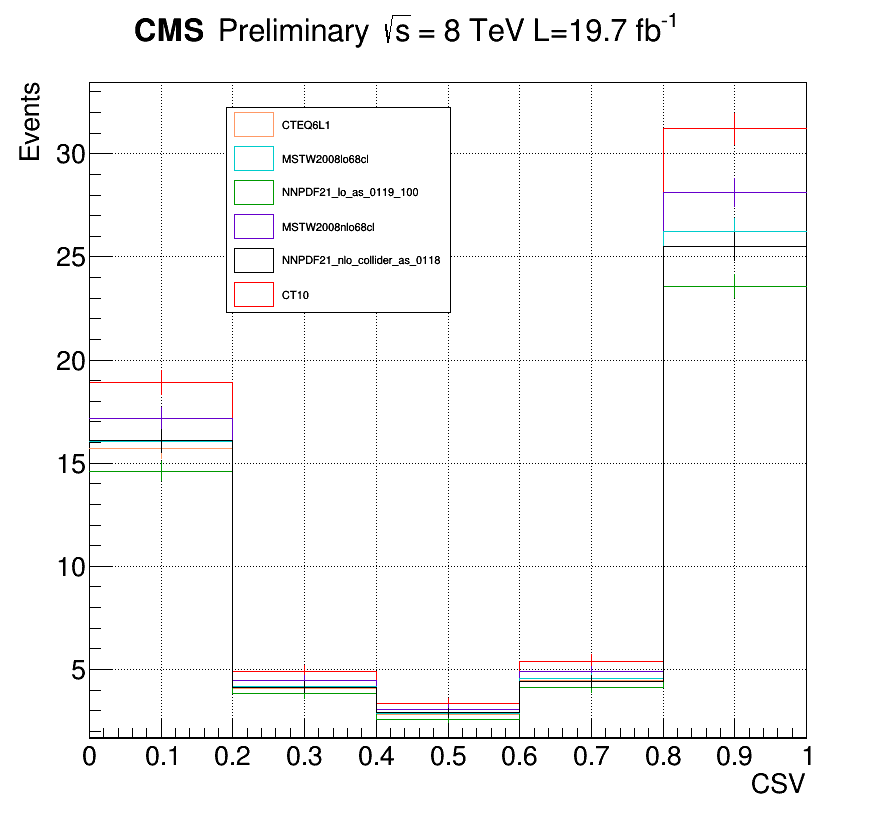
\includegraphics[scale=0.22]{figure/CH3/Systematics/StackCSV_M800.png}}
  \hspace{0.5cm}
  \subfigure[$m_{Zh}$ spectrum of 1200 GeV $Z'$ sample]{
    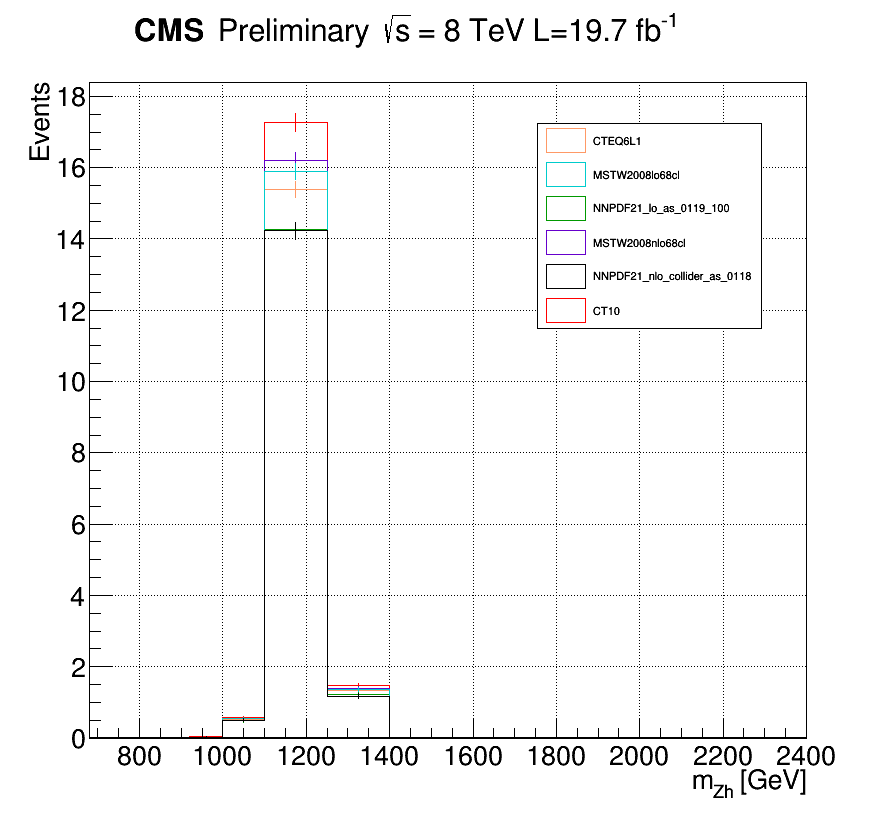
\includegraphics[scale=0.22]{figure/CH3/Systematics/StackPDF_M1200.png}}
  \hspace{0.5cm}
  \subfigure[$m_{Zh}$ spectrum of 2000 GeV $Z'$ sample]{
    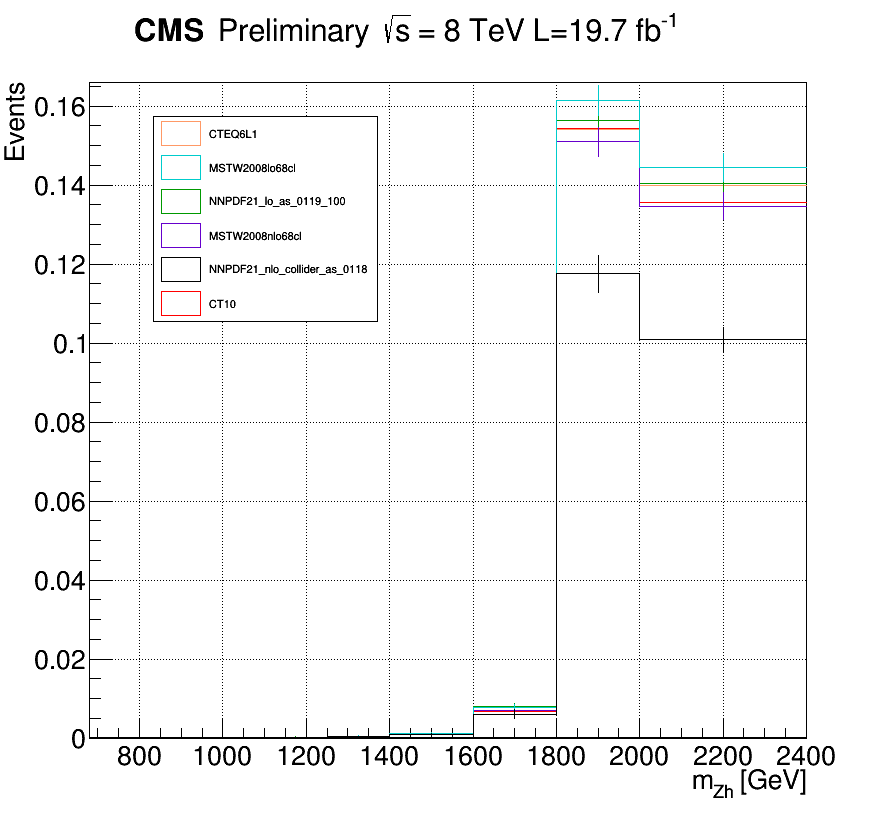
\includegraphics[scale=0.22]{figure/CH3/Systematics/StackPDF_M2000.png}}
  \caption{\label{fig:StackPDF} The comparison between different PDF sets using $m_{Zh}$ spectrum and CSV variable.}
\end{figure}
